% Klassifiziert den Dokumenten-Typ
% Doku: http://exp1.fkp.physik.tu-darmstadt.de/tuddesign/
% Farben: http://www.tu-darmstadt.de/media/medien_stabsstelle_km/services/medien_cd/das_bild_der_tu_darmstadt.pdf
%  bigchapter: Chapter haben doppelte Schriftgröße
%  linedtoc: Linien im Inhaltsverzeichnis wie bei Überschriften
%  colorbacktitle: Der Dokumenten-Titel wird mir der Accentfarbe hinterlegt
\documentclass[bigchapter,colorback,accentcolor=tud4b,linedtoc,11pt]{tudreport}

% Input Dokument hat das Encoding UTF-8
\usepackage[utf8]{inputenc}
% Wichtiges Paket für Links und verlinktes Inhaltsverzeichnis
\usepackage[ngerman]{hyperref}
% Paket für Fußnoten
\usepackage[stable]{footmisc}
% Paket für Bibliotheks-Verzeichnis, square: Verwende eckige statt runde klammern
% \usepackage[square]{natbib}
% Paket zum Plotten von Datensätzen
\usepackage{pgfplots}
% Verwende deutsche Bezeichner für Inhaltsverzeichnis, ... (ngerman = New German: neue Rechtschreibung)
\usepackage{ngerman}
% Modul für chemische Formeln
%\usepackage{chemformula}
% Deutsche Zahlen (entfernt z.B. das Leerzeichen nach einem Dezimal-Komma)
\usepackage{ziffer} 

\usepackage[verbose]{placeins}

%\usepackage{graphicx}
%\usepackage{caption}
\usepackage{subcaption} %Für subfigures

% PDF-Optionen
\hypersetup{
  pdftitle={TU Darmstadt \- Physikalisches Praktikum für Fortgeschrittene},
  pdfauthor={Esra Bauer und Sören Link},
  pdfsubject={Versuch 4.10},
  pdfview=FitH,
}

% Kleines makro zur assymetrischen Fehlerangabe
\def\tol#1#2#3{\hbox{\rule{0pt}{15pt}${#1}^{+{#2}}_{-{#3}}$}}% 

% Entspricht-Zeichen
\usepackage{scalerel}

\newcommand\equalhat{%
\let\savearraystretch\arraystretch
\renewcommand\arraystretch{0.3}
\begin{array}{c}
\stretchto{
    \scalerel*[\widthof{=}]{\wedge}
    {\rule{1ex}{3ex}}%
}{0.5ex}\\ 
=%
\end{array}
\let\arraystretch\savearraystretch
}
%BEGINN TITELSEITE

\title{Akusto-optischer Modulator}

\subtitle{Esra Bauer  \\Sören Link}

\subsubtitle{Betreuer: Daniel Schraft \hfill Versuchsdatum: 8. Dezember 2014}

\author{Esra Bauer, Sören Link}

%\settitlepicture{img/title.jpg}

\institution{Physikalisches Praktikum \\für Fortgeschrittene \\ Versuch 4.10}

\date{\today}


%ENDE TITELSEITE

\begin{document}
%ANFANG DOKUMENT

%Titelseite einfügen
\maketitle

%Inhaltsverzeichnis einfügen
\tableofcontents

%ANFANG INHALT

\chapter{Einleitung}

In diesem Versuch soll der akusto-optische Effekt untersucht werden und durch die Inbetriebnahme eines akusto-optischen Modulators auf verschiedene Arten angewendet werden. Entscheidend ist dabei die Wechselwirkung von Licht- und Schallwellen (im Versuch werden Ultraschallwellen eingesetzt), die es ermöglicht, dass Licht an Schallwellen wie an einem Kristall gebeugt wird. Akusto-optische Modulatoren sind heute u.a. wichtige Elemente der Forschung (z.b. Spektroskopie, Bose-Einstein-Kondensation) und der Telekommunikation sowie der Quantenoptik, um nur einige Einsatzgebiete zu nennen. Es können auch Laserpulse erzeugt werden und vieles mehr, was teilweise im Versuch umgesetzt bzw. aufgezeigt wird.

\chapter{Grundlagen}
\section{Akusto-optischer Effekt}

Der akusto-optische Modulator (AOM) nutzt die Tatsache, dass Schallwellen in einem Medium ein optisches Gitter erzeugen. Sie bewirken eine periodische Dichte- und somit Brechnungsindexmodulation, d.h. es entsteht ganz analog zur Bragg-Reflexion ein Gitter mit der ``Gitterkonstanten'' $\lambda_S$, der Schallwellenlänge. Es gilt folglich für konstruktive Interferenz: 
$$2~sin(\theta) = \frac{\lambda}{\lambda_S}$$ 
Zur technischen Umsetzung dient ein an einen Würfel montierter Piezo-Aktor, welcher beim Anlegen einer geeigneten Hochfrequenzspannung entsprechende mechanische Schwingungen ausführt. Auf der gegenüberliegenden Seite ist ein Absorber zur Verhinderung stehender Wellen angebracht.

\section{Betriebsregime eines AOM}

Die Bragg-Bedingung setzt bei genauer Betrachtung eine hinreichende Länge des Mediums voraus, durch welches die Schallwelle propagiert und eine Brechungsindexmodulation bewirkt. Es tritt dann nur die erste Beugungsordnung auf und man spricht vom Bragg-Regime. Dies liegt auch unserer Betrachtung zugrunde, man muss aber beachten, dass auch das sog. Raman-Nath (häufig auch: Debye-Sears-Regime) vorliegen kann, vor allem wenn die Länge des Mediums kurz im Vergleich zur Schallwellenlänge ist. Die Bragg-Bedingung gilt dann nicht mehr, d.h. es tritt keine klassische Beugung am Gitter auf, sondern lediglich eine periodische Veränderung der Phase des Lichts. Es sind dann auch höhere Beugungsordnungen zu beobachten. Zur Unterscheidung kann ein Parameter $\rho$ wie folgt definiert werden: 
$$\rho = \frac{\lambda_0^2}{\lambda_S~\bar{n}~n_1}$$
$\lambda_0$ ist dabei die Lichtwellenlänge im Vakuum, $\bar{n}$ der mittlere Brechnungsindex und $n_1$ die Modulation des Brechnungsindex. Gilt $\rho \gg 1$ (etwa ab 10), kann man vom Bragg-Regime ausgehen, für $\rho \leq 1$ vom Raman-Nath-Regime.

\section{Doppelpasskonfiguration}

Bei der Doppelpasskonfiguration ist das Entscheidende, dass das Laserlicht den AOM zweimal passiert. Der abgelenkte Strahl wird also reflektiert und fällt auf den AOM zurück. Da er beide Male um den gleichen Betrag abgelenkt wird, fällt der reflektierte Strahl wieder in den ursprünglichen zurück. Um den Strahl unabhängig vom einfallenden Strahl detektieren zu können, bedienen wir uns eines $\frac{\lambda}{4}$-Plättchens, welches zwischen AOM und Spiegel montiert wird. Dadurch wird die Polarisationsebene des einfallenden Strahls um insgesamt 90$^{\circ}$ gedreht und kann so mittels eines Polarisations-Strahlteilers separiert werden. Wichtig dabei ist, eine Linse in den Strahlengang zwischen Spiegel und AOM derart zu montieren, dass die Brennweite im AOM liegt. Andernfalls wäre es nicht möglich, dass die Strahlen senkrecht auf den Spiegel auftreffen und sie würden unkontrolliert abgelenkt.

Der Vorteil der Doppelpasskonfiguration liegt zum einen darin, dass die Bandbreite der Modulation erhöht wird und zum andern darin, dass kein Nachjustieren erforderlich ist, falls die Modulation geändert wird. Der modulierte Strahl läuft nämlich immer im einfallenden zurück bzw. wird dann vom Polarisations-Strahlteiler immer in gleicher Weise erfasst.

\section{Schwebungen}

Schwebungen entstehen bei der Überlagerung zweier Schwingen mit nur gering unterschiedlichen Frequenzen. Je kleiner die Differenz der Frequenz, desto deutlicher ist die Schwebung wahrzunehmen. Es entsteht eine langsame Cosinusschwingung der Frequenz $\omega_S = \frac{\omega_1 - \omega_2}{2}$, die die Einhüllende der Sinusschwingung der Frequenz $\omega = \frac{\omega_1 + \omega_2}{2}$ ist. Für den Versuch ist vor allem die Schwebung zwischen den Strahlen $\pm 1$. Ordnung von Bedeutung, da die Schwebungsfrequenz $f_S = |f_1 - f_2|$ zwischen ihnen gemessen werden kann und somit die Schallfrequenz bzw. -wellenlänge im AOM berechnet werden kann.

\section{Lissajous-Figuren}

Lissajous-Figuren sind Kurvengraphen, die aus der Überlagerung zweier harmonischer, senkrecht zueinander stehender, Schwingungen entstehen. Seien $\omega_1$, $\omega_2$ die Frequenzen dieser beiden Schwingungen, dann stellt man fest, dass für nicht ganz genau rationale Verhältnise $\frac{\omega_1}{\omega_2}$ der Eindruck einer Drehung der resultierenden Lissajous-Figur entsteht. Ist die Frequenz der senkrecht orientierten Schwingung höher, findet die Rotation um die waagerechte Achse statt und umgekehrt. Die Rotation wird für geringe Abweichungen vom rationalen Verhältnis langsam, für höhere Abweichungen schneller. Die Form der Figuren erlaubt Rückschlüsse auf Frequenz und Phasenlage der Schwingungen, weshalb sie für die Signalanalyse von Bedeutung sind.

\section{Gefahren durch Laserstrahlung und Vorsichtsmaßnahmen} %folgende Inhalte aus 4.9

Bei dem in diesem Versuch vorliegenden HeNe Laser mit einigen mW Leistung im roten Spektralbereich sind die potentiellen Gefahren durch Laserstrahlung überschaubar. Vor allem muss hier darauf geachtet werden, dass der Laser nicht in ein Auge gelangt. Aus diesem Grund ist bei eingeschaltetem Laser immer eine Schutzbrille zu Tragen und der Kopf ist nie auf Höhe des Lasers zu halten. Auch sollte darauf geachtet werden, dass Reflexe des Lasers wenn möglich auf die Laserapparatur selbst zurückgelenkt werden und vor allem nicht auf einen Eingang zeigen, da sonst Außenstehende ohne Schutzbrille gefährdet werden können.

Bei Lasern mit höherer Intensität ist zudem der Kontakt mit dem Körper zu vermeiden, da ein Laser nicht nur oberflächliche Verbrennungen, sondern im Falle eines UV-Lasers auch Hautkrebs und im Falle eines IR-Lasers schmerzlose und deswegen schwer zu erkennende Verbrennungen im Unterhautgewebe verursachen können. Zur Sichtbarmachung von Lasern sollte deswegen nie die nackte Haut sondern eine nicht reflektierende Oberfläche (beispielsweise ein Schirm, der die verwende Laserleistung aushält) verwendet werden.

Abgesehen von den genannte Personenschäden sind bei nicht sachgemäßer Handlung von Lasern mit hoher Intensität auch Schäden am Versuchsaufbau möglich. Verschmutzte Spiegel oder Fenster des Lasermediums können zu extremer Hitzeentwicklung an jeweiligen Material und letztendlich zu dessen Ermattung oder gar Zerstörung führen. \cite{GefahrenLaser}

\chapter{Durchführung und Auswertung} %pro section kurze Schilderung Versuchsaufbau, Durchführung u. Auswertung ggf. mit subsections

\section{Bauteile zur akusto-optischen Modulation}

Im Wesentlichen benötigt man zur Beobachtung des akusto-optischen Effektes eine geeignete Lichtquelle, den AOM samt geeigneter Stromquellen sowie einen Photodetektor und Auslesegerätschaft (Oszilloskop, Software). Als Lichtquelle nutzen wir einen He-Ne-Laser, der unpolarisiertes rotes Licht einer Wellenlänge von 633 nm mit einer Ausgangsleistung von 10 mW aussendet. Um die Ausgangsleistung zu variieren, nutzen wir daher zusätzlich einen Polarisator. Außerdem ist ein Polarisations-Strahlteiler (PBS) vorhanden, mit dem ebenfalls die Intensität des Lichts variiert werden kann und der später für die Doppelpasskonfiguration wichtig ist. Weiterhin sind zwei baugleiche AOMs vorhanden, wobei einer horizontal, der andere vertikal ablenkt. IdR. wird der horizontal ablenkende AOM zur Verwendung gebracht. Zur Inbetriebnahme der AOMs wird eine geeignete Hochfrequenz-Spannungsversorgung benötigt. Diese erhalten wir für jeden AOM aus einem sog. Voltage Controlled Oszillator (VCO), welcher die Frequenz der Schallwelle über einen Frequenzmodulationseingang (FREQ IN) mit Spannungsn $U_F$ zwischen 0 V und 10 V regeln kann und die Amplitude über einen Modulationseingang (MOD IN) mit Spannungen $U_M$ zwischen 0 V und 5 V. Da das Piezoelement der AOMs eine sehr viel höhere Leistung benötigt als durch die VCOs bereitgestellt werden kann, werden zusätzlich Verstärker zwischengeschaltet. VCOs und Verstärker werden mit einer Spannung von 24 V von einem Labornetzteil versorgt. Die Steuerspannungen $U_F$ und $U_M$ für die VCOs erzeugen wir mit zwei Funktionsgeneratoren, mit denen man DC-, Rechteck-, Sinus-, Sägezahn- und Pulsspannungen erzeugen kann. Die Einstellung erfolgt direkt über Knöpfe oder über Ansteuerung via PC.

Zur Messung der Intensität des gebeugten Lichts ist ein Photodektor mit einer Photodiode vorhanden, der an ein Oszilloskop angeschlossen wird, um die Messwerte als Spannungen über der Zeit sichtbar zu machen. Das Oszilloskop kann ebenfalls über den PC verwendet werden, da es über einen USB-Anschluss verfügt. Zusätzlich ist ein Spektralanalysator vorhanden, der die Ausgangswerte des Photodetektors bis zu einer Frequenz von 1 GHz darstellen kann, sowie eine CCD-Kamera, die mit dem PC verbunden wird und zum Abspeichern von Bildern (z.B. der Lissajous-Figuren) dient.

\section{Inbetriebnahme des AOMs}

Zunächst soll der AOM in Betrieb genommen werden und die erste Beugungsordnung sichtbar gemacht werden. Der AOM, der Polarisator, der Polarisations-Strahlteiler sowie der Photodetektor werden vor den Laser entsprechend folgender Skizze aufgebaut:

\begin{figure}[h] 
  \centering
     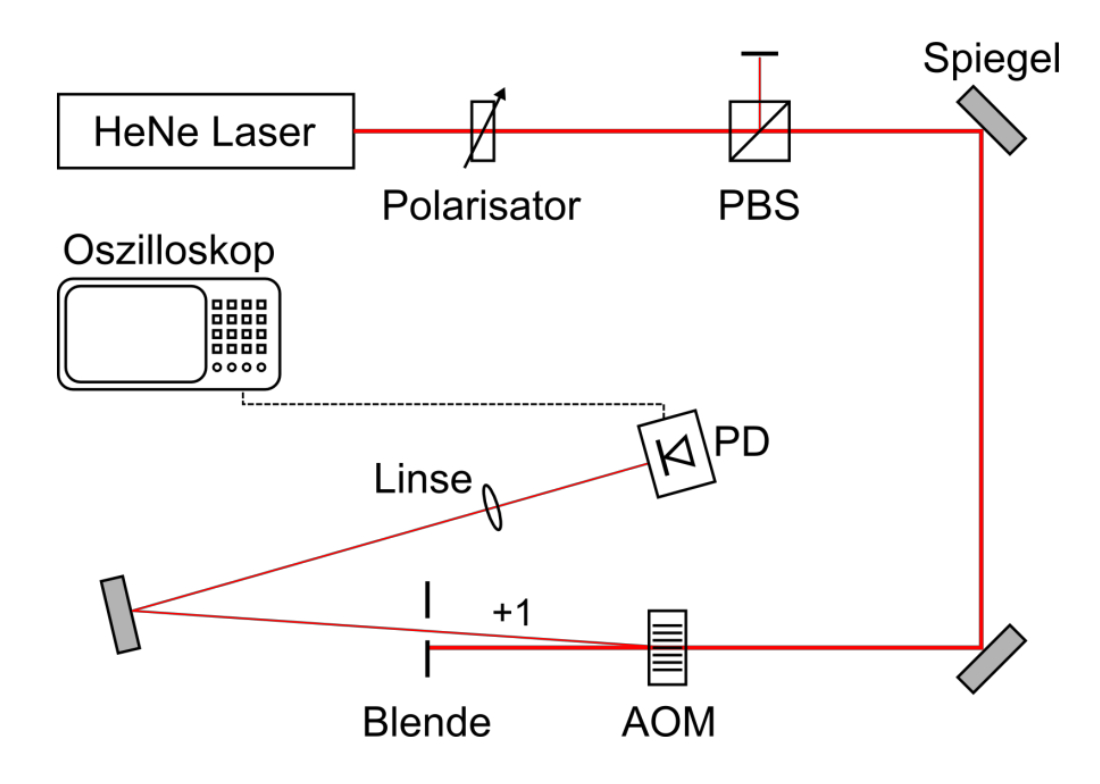
\includegraphics[width=0.7\textwidth]{data/inbetriebnahme.jpg}
  \caption[Cap for listoffigures]{Aufbau zur Detektierung der ersten Beugungsordnung \cite{Anleitung}}
  \label{fig:Bild1}
\end{figure}

Alle Komponenten werden nacheinander so ausgerichtet, dass der Strahl durchgehend möglichst auf der gleichen Höhe (ca. 10 cm) horizontal über dem Tisch verläuft. Bei Installation einer Komponente wird zunächst der Strahl abgeblockt und sichergestellt, dass keine unkontrollierten Reflexe auftreten. Um den Versuchsaufbau nicht zu groß werden zu lassen, wird der Strahl mehrfach mit Spiegeln umgelenkt. Die Linse ist notwendig, um den leicht divergenten Strahl vollständig auf die Fläche der Photodiode abbilden zu können. Mittels der Blende blockieren wir die nullte Beugungsordnung sowie die höheren Beugungsordnungen, so dass die Messung mit dem Photodetektor nur die erste Ordnung erfasst.

\section{Beugungseffizienz in Abhängigkeit der Schallintensität}

Es soll nun die Beugungseffizienz $\epsilon = \frac{I_1}{I_{einfallend}}$ bestimmt werden, d.h. der Quotient aus der Intensität des ersten Beugungsmaximums und der gesamten einfallenden Intensität. Dazu wird der Messaufbau unverändert gestartet, wobei nun über ein eigens geschriebenes Computerprogramm die Frequenzgeneratoren und das Oszilloskop derart angesteuert werden, dass jeweils für eine feste Spannung $U_F$ eine Variation von $U_M$ in 0,1 V-Schritten von 0 V bis 5 V erfolgt und die Werte ausgezeichnet werden. $U_F$ verstellen wir von Hand in 1 V-Schritten von 0 V bis 10 V, so dass wir 10 Messreihen mit Werten für die Intensität der ersten Beugungsordnung erhalten. Zu beachten ist das unterschiedliche Offset der Photodiode, welches ohne Streulicht stets 12 mV beträgt und mit Streulicht 16 mV für die zweite Messreihe und 160 mV für alle anderen Messreihen. Dies kommt durch das bei der zweiten Messreihe geschlossene Rollo im Versuchsraum zustande (bedingt durch die Messung einer anderen Laborgruppe). Zusätzlich ist der Laser thermisch nicht völlig stabil, was sich in einer Schwankung des Messwertes für die nullte Begungsordnung von 7,6 V bis 8,16 V bemerkbar macht.

\section{Beugungseffizienz in Abhängigkeit des Winkels}

\section{Pulserzeugung}

\section{AOM als Frequenzschieber}

\section{AOM als Deflektor}

\chapter{Fazit}

%ENDE INHALT
\cleardoublepage{}
% Eintrag fürs Inhaltsverzeichnis
\newpage
\begin{thebibliography}{100}
   \bibitem{GefahrenLaser} \url{http://de.wikipedia.org/w/index.php?title=Laser&oldid=128632514#Gefahren}
   
   \bibitem{Anleitung} Anleitungsblatt zum Versuch
\end{thebibliography}

\cleardoublepage{}
% Eintrag fürs Inhaltsverzeichnis
% Abbildungsverzeichnis einfügen
\end{document}
